% Angabe zu Blattgröße, Schriftgröße, Hinzufügen des Bildverzeichnis und Quellverzeichnis als Punkt im Inhaltsverzeichnis, einseitiger Druck
\documentclass[a4paper,12pt,listof=toc,bibliography=totoc,oneside, titlepage, headsepline,headings=optiontohead]{scrartcl}
\usepackage[table]{xcolor}
\usepackage{geometry}
\usepackage[utf8]{inputenc} % Zeichenkodierung
\usepackage[ngerman]{babel} %Sprachpaket
\usepackage{blindtext}
\usepackage{csquotes}
\usepackage{graphicx}
\usepackage{amssymb}
\usepackage{enumitem,xcolor}
\usepackage{xpatch}
\usepackage{tabularx}
%Verlinkungen inner- und außerhalb von Latex
\usepackage[pdftex]{hyperref}
\usepackage[hyperref]{ntheorem}
\usepackage[automark]{scrlayer-scrpage}
\usepackage{titletoc}
%Grafik und Grafikpositionierung
\usepackage{graphicx}
\usepackage{here}
\usepackage[export]{adjustbox}
\usepackage[many]{tcolorbox}
\usepackage{framed}
\usepackage[strict]{changepage}
\graphicspath{{img/}}
\usepackage{rotating}
\usepackage{fancyvrb}
\usepackage{relsize}
\usepackage{multirow}
\usepackage{float}

%-- colorize blindtext--
\LetLtxMacro{\blindtextblindtext}{\blindtext}
\RenewDocumentCommand{\blindtext}{O{\value{blindtext}}}{%
  \begingroup\color{red}\blindtextblindtext[#1]\endgroup
}

%Seitenränder
\geometry{a4paper, top=30mm, left=20mm, right=20mm, bottom=25mm, headsep=10mm, footskip=15mm}

%THM-Farben
\definecolor{thm_green}{cmyk}{0.57,0,1,0}
\definecolor{thm_grey}{cmyk}{0.33, 0.04, 0, 0.72}
\definecolor{thm_red}{cmyk}{0, 1, 0.65, 0.28}
\definecolor{thm_yellow}{cmyk}{0,0.30,1,0}
\definecolor{thm_lightblue}{cmyk}{0.75,0,0.07,0}
\definecolor{thm_blue}{cmyk}{0.1,0.72,0,0.18}
\definecolor{thm_lightGray}{cmyk}{0.07,0,0,0.12}

% Kopf - und Fusszeile
\clearpairofpagestyles
\ihead{\leftmark}
\addtokomafont{headsepline}{\color{thm_green}}
\cfoot*{\pagemark}

%=========== Zitate ===========================================================%

\newenvironment{formal}{%
  \def\FrameCommand{%
    \hspace{1pt}%
    {\color{thm_grey}\vrule width 5pt}%
    {\color{thm_grey!10}\vrule width 4pt}%
    \colorbox{thm_grey!10}%
  }%
  \MakeFramed{\advance\hsize-\width\FrameRestore}%
  \noindent\hspace{-4.55pt}% disable indenting first paragraph
  \begin{adjustwidth}{}{7pt}%
  \vspace{2pt}\vspace{2pt}%
}
{%
  \vspace{2pt}\end{adjustwidth}\endMakeFramed%
}

%===== Bildherkunft =========================
\newcommand{\captionsource}[1]{\itshape\footnotesize (#1)}

% Deckblatt
\makeatletter
\AtBeginDocument{\hypersetup{
	pdftitle={\@title},
	% pdfsubject={\@subtitle},
	% pdfauthor={\@author},
	bookmarksopen=true,
	bookmarksopenlevel=3,
	breaklinks,
	colorlinks,
	citecolor=red,
	linkcolor=black,
	urlcolor=black,
}}

\newcommand*{\institute}[1]{\gdef\@institute{#1}}
\newcommand*{\@institute}{}%

\newcommand*{\mail}[1]{\gdef\@mail{#1}}
\newcommand*{\@mail}{}%

\renewcommand*{\maketitle}{%
  \global\@topnum=\z@
  \setparsizes{\z@}{\z@}{\z@\@plus 1fil}\par@updaterelative
  \null
  \vskip 4em%
  \begin{center}%
    \ifx\@subject\@empty \else
      {\usekomafont{subject}{\@subject \par}}%
      \vskip 1.5em
    \fi
    {\usekomafont{title}{\huge \@title \par}}%
    \vskip .5em
    {\ifx\@subtitle\@empty\else\usekomafont{subtitle}\@subtitle\par\fi}%
    \vskip 5em
    {%
      \usekomafont{author}{%
        \lineskip .5em%
        \begin{tabular}[t]{@{}c}
          \@author
        \end{tabular}\par
      }%
    \vskip .5em
    }%
	{\texttt\@mail\par}
    \vfill
    {\usekomafont{publishers}{\@publishers \par}}%
	\vfill
    {\usekomafont{publishers}{\large\@date\\Technische Hochschule Mittelhessen, Gießen \par}}
  \end{center}%
  \par
  \vskip 2em
}%

\renewcommand{\arraystretch}{1.5}
\setlength{\arrayrulewidth}{0.7mm}

\makeatother

\usepackage{tikz}
\newcommand*\circled[1]{\tikz[baseline=(char.base)]{
            \node[shape=circle,draw,inner sep=2pt] (char) {#1};}}
\usepackage{enumitem}
\usepackage{mathtools}
\usepackage{listings}

\subject{
CS2018 Entwicklung mobiler Anwendungen WS2022/23}
\title{Projektbericht}
\subtitle{Gruppe 8}
\author{
  Biebl, Maximilian\\
  Wagner, Hendrik\\
  Krs, Dennis\\
  Nagy, Vanessa\\
  Thomas, Sven\\
}
\publishers{
  Dozent:\\
  Prof. Dr. Steffen Vaupel\\
  \vspace{1cm}
  }

\lstset{
  basicstyle=\footnotesize\ttfamily,
  breaklines=true,
  breakatwhitespace=true,
  captionpos=b,
  commentstyle=\color{blue},
  deletekeywords={...},
  escapeinside={\%*}{*)},
  extendedchars=true,
  frame=single,
  keepspaces=true,
  keywordstyle=\color{blue}
}

% % % % % % % % % % % % % %
% % % Dokument Beginn % % %
% % % % % % % % % % % % % %
\begin{document}
%Deckblatt
\begin{titlepage}
	\begin{minipage}[t]{\textwidth}
		\vspace{-1cm}
		
\includegraphics[height=20mm]{mni-logo.pdf}
		\hspace{59mm}
	  \end{minipage}
  	\vspace{1cm}
	\maketitle
\end{titlepage}

%Inhaltsverzeichnis
\pagenumbering{roman}
\tableofcontents
\clearpage

%Inhalt
\pagenumbering{arabic}
\pagestyle{scrheadings}
\setcounter{page}{1} %Seitenzähler auf 1 setzen, da Inhaltsverzeichnis sonst als Seite 1 zählt
\section{Einleitung}

Auf den folgenden Seiten befindet sich der ausführliche Projektbericht zur App \enquote{Almanify}.
In diesem Bericht werden die Anforderungen, die Entwicklungsprozesse und die Ergebnisse unserer Arbeit detailliert beschrieben.
Es wird auch auf die Herausforderungen eingegangen, mit denen das Entwicklungsteam während der Entwicklung konfrontiert wurden, und wie sie sie gelöst haben.
Zudem werden die Funktionen und Möglichkeiten der App aufgezeigt und eine Übersicht über die Ergebnisse der Entwicklung und der Benutzertests präsentiert.

\subsection{Problem und Zielsetzung}

Auf einer Reise mit mehreren Beteiligten kommt es oft vor, dass sich Teilnehmer gegenseitig Geld vorlegen, um eine Bezahlung zu vereinfachen.
Schnell kann es dabei unübersichtlich werden, insbesondere bei einem Roadtrip mit mehreren Freunden,
bei dem jeder für etwas anderes bezahlt und man nicht immer eine klare Übersicht hat.
Einer kauft noch schnell ein paar Snacks für alle, der andere fährt zwischendurch das Auto tanken,
und jemand hat kein Bargeld, um dem Fremdenführer Trinkgeld zu geben.
Daher muss er sich das Geld leihen.
Die App \enquote{Almanify} soll dabei helfen, diese komplexe Situation zu vereinfachen, indem alle Beteiligten die Ausgaben transparent miteinander verwalten können.
Am Ende sowie während der Reise soll es den Nutzern möglich sein, offenen Schulden gegenüber Mitreisenden einzusehen, um diese begleichen zu können.

\subsection{Anforderungen}

Bei Öffnung der App müssen sich Benutzer zunächst einloggen oder registrieren.
Dann können Sie Reisen erstellen und andere Nutzer über einen Invitecode oder QR-Code einladen.
Ausgaben im Rahmen einer Reise können hinzugefügt werden.
Beim Erstellen von Ausgaben gibt vorgegebene Auswahlmöglichkeiten für Währung, Kategorie und Beteiligte.
Nutzer können Einträge bearbeiten und Schulden gegenüber anderen auswerten.
Die App schlägt einen effizienten finanziellen Ausgleich vor und Schulden werden in eine vom User gewählte Währung umgerechnet.
Nach Abschluss einer Reise kann dies archiviert werden.

\subsection{Ausgewählte Technologien}

Die Anwendung basiert auf Angular.
Als Framework für die Implementierung der mobilen Anwendung kommt Ionic zum Einsatz.
Firebase dient als Backend für die Datenhaltung und Nutzerverwaltung.

Wir beschränken uns bei der Implementierung der nativen Komponenten der App auf die Android-Plattform.

\pagebreak

\subsection{Organisation und Vorgehensmodell}

Die Gruppe wurde zunächst mit einem ausführlichen Kickoff-Meeting, welches schon erste Mockups enthielt, vom Ideengeber über das Konzept der App aufgeklärt.
Im Anschluss an das Kickoff-Meeting wurden grundsätzliche Features und Designentscheidungen anhand der Mockups besprochen.

Im laufenden Projekt wurde sich an Scrum orientiert.
Die Sprints dauerten eine Woche.
Das Team traf sich jeden Mittwoch in Discord, um die Features der vorherigen Woche zu besprechen und zu sehen, wo Verbesserungen nötig waren.
Außerdem wurde diskutiert, welche Features in der kommenden Woche implementiert werden sollten.

\section{Anforderungen}

Bei Öffnung der App können sich Benutzer einloggen oder registrieren. Dabei wird ein Benutzerprofil erstellt, das den Nutzernamen enthält. Reisen können innerhalb der mobilen Anwendung erstellt werden. Weitere Nutzer können über einen Invitecode oder QR-Code beitreten. Getätigte Ausgaben können den beigetretenen Reisen hinzugefügt werden. Einträge für Ausgaben umfassen einen Titel, die Person, die bezahlt hat, die Summe, Währung, eine Kategorie, Zahldatum, die Beteiligten, die Ausgaben verursacht haben, eine optionale Markierung auf Google Maps wo die Zahlung getätigt wurde und ein optionales Bild vom Kassenbon. Für Währung, Kategorie und Beteiligte gibt es vorgegebene Auswahlmöglichkeiten. Einträge für Ausgaben können entsprechend der Attribute sortiert werden. Nutzer können Einträge für Ausgaben nachträglich bearbeiten. Es ist möglich, Schulden bzw. Ansprüche gegenüber anderen auszuwerten. Die App schlägt einen effizienten finanziellen Ausgleich unter den Beteiligten vor, sodass möglichst wenige Transaktionen nötig sind. Schulden des Nutzers gegenüber anderen werden in eine von ihm angegebene Währung umgerechnet. Nach Abschluss einer Reise kann dies archiviert werden.

\subsection{Grundlegende Funktionsbeschreibung}

Funktionsbeschreibung anhand von User Stories:

\begin{table}[H]
\caption{Account erstellen}
\begin{tabularx}{0.95\textwidth}{ |X|X| }
\hline
\rowcolor{gray} \textbf{Abschnitt} & \textbf{Inhalt} \\
\hline
	Primärer Akteur (Initiator) & Nutzer \\
\hline
	Weitere Akteure & - \\
\hline
	Auslösende Ereignisse (Trigger) & [--TODO--] \\
\hline
\rowcolor{lightgray} \textbf{Szenario} & \textbf{Beschreibung} \\
\hline
	Hauptszenario & [--TODO--] \\
\hline
  	Alternativszenarien & [--TODO--] \\
\hline
  	Ausnahmeszenarien & [--TODO--] \\
\hline
\rowcolor{lightgray} & \\
\hline
  	Vor-/ Nachbedingungen & [--TODO--] \\
\hline
\end{tabularx}
\end{table}


\begin{table}[H]
\caption{In Account einloggen}
\begin{tabularx}{0.95\textwidth}{ |X|X| }
\hline
\rowcolor{gray} \textbf{Abschnitt} & \textbf{Inhalt} \\
\hline
	Primärer Akteur (Initiator) & Nutzer \\
\hline
	Weitere Akteure & - \\
\hline
	Auslösende Ereignisse (Trigger) & [--TODO--] \\
\hline
\rowcolor{lightgray} \textbf{Szenario} & \textbf{Beschreibung} \\
\hline
	Hauptszenario & [--TODO--] [Beitritt via Invitecode] \\
\hline
  	Alternativszenarien & [--TODO--] [Beitritt via QR-Code]\\
\hline
  	Ausnahmeszenarien & [--TODO--] \\
\hline
\rowcolor{lightgray} & \\
\hline
  	Vor-/ Nachbedingungen & [--TODO--] \\
\hline
\end{tabularx}
\end{table}


\begin{table}[H]
\caption{Eine Reise erstellen/beitreten}
\begin{tabularx}{0.95\textwidth}{ |X|X| }
\hline
\rowcolor{gray} \textbf{Abschnitt} & \textbf{Inhalt} \\
\hline
	Primärer Akteur (Initiator) & Reiseleiter \\
\hline
	Weitere Akteure & Reisemitglied \\
\hline
	Auslösende Ereignisse (Trigger) & [--TODO--] \\
\hline
\rowcolor{lightgray} \textbf{Szenario} & \textbf{Beschreibung} \\
\hline
	Hauptszenario & [--TODO--] [Normales Einloggen] \\
\hline
  	Alternativszenarien & [--TODO--] ['Remember Me' Einloggen]\\
\hline
  	Ausnahmeszenarien & [--TODO--] \\
\hline
\rowcolor{lightgray} & \\
\hline
  	Vor-/ Nachbedingungen & [--TODO--] \\
\hline
\end{tabularx}
\end{table}


\begin{table}[H]
\caption{Zahlung festhalten}
\begin{tabularx}{0.95\textwidth}{ |X|X| }
\hline
\rowcolor{gray} \textbf{Abschnitt} & \textbf{Inhalt} \\
\hline
	Primärer Akteur (Initiator) & Reisemitglied \\
\hline
	Weitere Akteure & - \\
\hline
	Auslösende Ereignisse (Trigger) & [--TODO--] \\
\hline
\rowcolor{lightgray} \textbf{Szenario} & \textbf{Beschreibung} \\
\hline
	Hauptszenario & [--TODO--] \\
\hline
  	Alternativszenarien & [--TODO--] \\
\hline
  	Ausnahmeszenarien & [--TODO--] \\
\hline
\rowcolor{lightgray} & \\
\hline
  	Vor-/ Nachbedingungen & [--TODO--] \\
\hline
\end{tabularx}
\end{table}


\begin{table}[H]
\caption{Zahlung einsehen}
\begin{tabularx}{0.95\textwidth}{ |X|X| }
\hline
\rowcolor{gray} \textbf{Abschnitt} & \textbf{Inhalt} \\
\hline
	Primärer Akteur (Initiator) & Reisemitglied \\
\hline
	Weitere Akteure & - \\
\hline
	Auslösende Ereignisse (Trigger) & [--TODO--] \\
\hline
\rowcolor{lightgray} \textbf{Szenario} & \textbf{Beschreibung} \\
\hline
	Hauptszenario & [--TODO--] \\
\hline
  	Alternativszenarien & [--TODO--] \\
\hline
  	Ausnahmeszenarien & [--TODO--] \\
\hline
\rowcolor{lightgray} & \\
\hline
  	Vor-/ Nachbedingungen & [--TODO--] \\
\hline
\end{tabularx}
\end{table}


\begin{table}[H]
\caption{Schulden einsehen}
\begin{tabularx}{0.95\textwidth}{ |X|X| }
\hline
\rowcolor{gray} \textbf{Abschnitt} & \textbf{Inhalt} \\
\hline
	Primärer Akteur (Initiator) & Reisemitglied \\
\hline
	Weitere Akteure & - \\
\hline
	Auslösende Ereignisse (Trigger) & [--TODO--] \\

\hline
\rowcolor{lightgray} \textbf{Szenario} & \textbf{Beschreibung} \\
\hline
	Hauptszenario & [--TODO--] \\
\hline
  	Alternativszenarien & [--TODO--] \\
\hline
  	Ausnahmeszenarien & [--TODO--] \\
\hline
\rowcolor{lightgray} & \\
\hline
  	Vor-/ Nachbedingungen & [--TODO--] \\
\hline
\end{tabularx}
\end{table}


\begin{table}[H]
\caption{Reise archivieren}
\begin{tabularx}{0.95\textwidth}{ |X|X| }
\hline
\rowcolor{gray} \textbf{Abschnitt} & \textbf{Inhalt} \\
\hline
	Primärer Akteur (Initiator) & Reiseleiter \\
\hline
	Weitere Akteure & - \\
\hline
	Auslösende Ereignisse (Trigger) & [--TODO--] \\

\hline
\rowcolor{lightgray} \textbf{Szenario} & \textbf{Beschreibung} \\
\hline
	Hauptszenario & [--TODO--] \\
\hline
  	Alternativszenarien & [--TODO--] \\
\hline
  	Ausnahmeszenarien & [--TODO--] \\
\hline
\rowcolor{lightgray} & \\
\hline
  	Vor-/ Nachbedingungen & [--TODO--] \\
\hline
\end{tabularx}
\end{table}


\begin{table}[H]
\caption{Reisen einsehen}
\begin{tabularx}{0.95\textwidth}{ |X|X| }
\hline
\rowcolor{gray} \textbf{Abschnitt} & \textbf{Inhalt} \\
\hline
	Primärer Akteur (Initiator) & Reisemitglied \\
\hline
	Weitere Akteure & - \\
\hline
	Auslösende Ereignisse (Trigger) & [--TODO--] \\

\hline
\rowcolor{lightgray} \textbf{Szenario} & \textbf{Beschreibung} \\
\hline
	Hauptszenario & [--TODO--] \\
\hline
  	Alternativszenarien & [--TODO--] \\
\hline
  	Ausnahmeszenarien & [--TODO--] \\
\hline
\rowcolor{lightgray} & \\
\hline
  	Vor-/ Nachbedingungen & [--TODO--] \\
\hline
\end{tabularx}
\end{table}


\subsection{Funktionale Anforderungen}

\subsection{ Nicht funktionale Anforderungen}

\subsection{(Benutzer) Schnittstellen / Ein-Ausgabeformate}

\subsection{Fehlverhalten}

\subsection{Abnahmekriterien}
\section{Entwurf}

\subsection{Technische Funktionen (und Funktionsabhängigkeiten)}

\subsection{Datenmodell}

\subsection{Strukturmodell (Aufbau)}

\subsection{Funktionsmodell (Verhalten)}

\subsection{Testfälle}
\section {Umsetzung}

\subsection{Schuldenberechnung}

Für die Schuldenberechnung musste zunächst ein Algorithmus entwickelt werden, der die Schulden berechnet innerhalb einer bestimmten Reise berechnet.
Es gab eine Reihe von Anforderungen an den Algorithmus, die erfüllt werden mussten:

\begin{itemize}
\item Der Algorithmus soll alle Zahlungen innerhalb der Reise berücksichtigen.
\item Hat Person A Person B zweimal Geld \emph{geliehen} (d. h. für diese Person eine Zahlung getätigt), sollen diese Zahlungen zusammengefasst werden.
\item Zahlungen können mehrere Personen betreffen, z. B. wenn eine Person für mehrere Personen bezahlt. In diesem Fall muss die Schuld aufgeteilt werden.
\item Die Anzahl an geforderten Ausgleichszahlungen soll minimiert werden.
\end{itemize}

Besonders der letzte Punkt verursachte Schwierigkeiten, da es sich hier um ein Optimierungsproblem handelt.
Ein Ansatz war es, die Zahlungen als einen Graphen zu modellieren, in dem die Knoten die Personen und die Kanten die Zahlungen darstellen.
Ausgehend von diesem Modell sollten dann Kanten vereinfacht werden. Dafür konnten einige Regeln aufgestellt werden:

\begin{enumerate}
    \item Transitiv: $x>y:A \xrightarrow{x} B \xrightarrow{y} C$ wird zu $A \xrightarrow{x-y} B$ und $A \xrightarrow{y} C$
    \item Transitiv 2: $x<y:A \xrightarrow{x} B \xrightarrow{y} C$ wird zu $A \xrightarrow{x} C$ und $A \xrightarrow{y-x} C$
    \item Transitiv 3: $x=y:A \xrightarrow{x} B \xrightarrow{y} C$ wird zu $A \xrightarrow{x} C$
    \item Reflexiv: $A \xrightarrow{x} A$ wird eleminiert (da die Person sich selbst nichts schuldet)
    \item Symmetrisch: $A \xrightarrow{x} B \xrightarrow{y} A$ wird zu $A \xrightarrow{x-y} B$ (bzw. $A \xleftarrow{y-x} B$)
    \item Kreise: Bei einem Kreis wird die kleinste Kante entfernt und die restlichen Kanten um den Betrag der entfernten Kante verkleinert
\end{enumerate}

Diese händische Vereinfachung stellte sich als übertrieben aufwändig heraus, als eine andere Idee aufkam:
Statt dem Zahlungsgraphen wird lediglich die Liste der Zahlungen betrachtet.
Für jede Person wird ein Wert verwaltet, auf welchen für jede Zahlung, in die der Person profitiert hat, der (Teil-)betrag subtrahiert wird.
Für jede Zahlung, die die Person selbst getätigt hat, wird der Betrag addiert. 

Mit diesen Werten wird dann wie in diesem Pseudocode beschrieben vorgegangen:

\begin{lstlisting}
sei P eine gefuellte Map [Person, Wert]
sei S eine leere Liste von zu begleichenden Schulden [Schuldner, Glaeubiger, Betrag]
sortiere P nach Werten aufsteigend
solange P nicht leer ist
    Person A = erste Person in P (Person mit kleinstem Wert, d.h. Person, die am meisten schuldet)
    Person B = letzte Person in P (Person mit groesstem Wert)
    Betrag = min(negiere(Wert von A), Wert von B)
    Fuege in S eine neue Schuld [A, B, Betrag] ein
    setze Wert von A auf Wert von A - Betrag
    setze Wert von B auf Wert von B + Betrag
    entferne A aus P, wenn Wert von A = 0
    entferne B aus P, wenn Wert von B = 0
\end{lstlisting}

Mit diesem Algorithmus werden die Schulden berechnet und in einer Liste gespeichert.
Diese Liste wird dann verwendet, um eventuell relevante Schulden dem Benutzer anzuzeigen.
Da der Algorithmus sehr simpel ist (Laufzeit $\mathcal{O}(n^2)$, generiert durch das Sortieren der Liste), genügt es, ihn auf Nachfrage im Client zu berechnen und die Schulden nicht im Server zu speichern.

\subsection{CRUD-Handler}

Die App kommuniziert mit mehreren Datenbanktabellen und muss daher für jede Tabelle einen eigenen Handler implementieren.
Um die Implementierung zu vereinfachen, wurde ein generischer Handler entwickelt, der die CRUD-Operationen für eine beliebige Tabelle erledigt.
Dieser Handler wird mit dem Namen der Tabelle initialisiert und kann dann die CRUD-Operationen für diese Tabelle ausführen.

\begin{enumerate}
    \item \textbf{createAndGetID}: Erstellt einen neuen Eintrag in der Tabelle.
    \item \textbf{readByID}: Liest einen Eintrag aus der Tabelle anhand der ID.
    \item \textbf{update}: Aktualisiert einen Eintrag in der Tabelle.
    \item \textbf{delete}: Löscht einen Eintrag aus der Tabelle.
\end{enumerate}

\subsection{Nichtumsetzung von Funktionen}

\subsubsection{Google-Maps Integration}

Die App sollte für eine Zahlung eine Karte anzeigen können, auf der die Position des Zahlungsortes angezeigt werden könnte.
Dafür sollte die App die Google Maps API verwenden.

Die Integration der Google Maps API in die App wäre jedoch sehr aufwändig gewesen -- so hätten wir neben der Darstellung auch die Möglichkeit der Suche nach Orten implementieren müssen.
Zudem müssten GPS-Daten gesammelt werden, um einen Zahlungsort sinnvoll vorzuschlagen.

Diese Funktion wurde nicht umgesetzt, da das Feature nicht zwingend notwendig war und in vielen Fällen keine sinnvollen zusätzlichen Daten liefern würde -- so ist z. B. der Name des Restaurants oft in der Zahlung als Titel angegeben.
Auch war der generierte Nutzen gering, da Nutzer wenig Nutzen für die Information haben, wo sie eine Zahlung getätigt haben.

\subsubsection{Währungs-API}

Die App sollte die Möglichkeit bieten, die Währung der Zahlungen zu ändern.
Dies wurde umgesetzt, nicht jedoch das Abrufen der aktuellen Wechselkurse.

Dies hatte mehrere Gründe:
\begin{enumerate}
    \item Die API, die wir für die Umrechnung der Währungen verwenden wollten, ist kostenpflichtig. Wir konnten keine kostenlose API finden, die die Wechselkurse aktuell hält.
    \item Die Schuldenbegleichung könnte durch die Umrechnung der Währungen verfälscht werden, da die Wechselkurse nicht aktuell sind. Dann könnte es z. B. nach einer Woche so aussehen, als ob ein Schuldner etwas zu viel oder zu wenig bezahlt hat, wenn die Wechselkurse sich in der Zwischenzeit geändert haben.
\end{enumerate}

\subsubsection{QR-Code-Scanner}

Die App sollte die Möglichkeit bieten, einer Reise mittels QR-Code beizutreten.
Die Generierung des QR-Codes wurde implementiert, jedoch nicht die Funktion, den QR-Code zu scannen.
Dies wurde nicht umgesetzt, da das Plugin für den QR-Code-Scanner nicht funktioniert hat und wir das Problem trotz Zuhilfenahme von Dokumentation und weiteren Quellen nicht lösen konnten.

\subsection{Designunterschiede unter Android und iOS}

Die App wurde hauptsächlich für Web und Android entwickelt.
Die iOS-Version wird beim Ionic-Framework automatisch generiert, das Styling wurde aber für Android angepasst.
Es wurden nachträglich einige Änderungen vorgenommen, um das Design auf iOS zu verbessern.
\section{Qualitätssicherung (Testprotokoll)} \label{Tests}

 	\subsection{Erläuterung der Userteststudie}
Um die Qualität zu gewährleisten, haben wir uns ein Studienkonzept überlegt. Dabei stellen wir unseren Probanden verschiedene Aufgaben in unserer App. Während sie die Aufgaben erfüllen, beobachten wir sie und bewerten ihre Leistungen mit vier möglichen Ausprägungen: 'sehr gut', 'gut', 'ok' und 'schlecht'. Wenn bei einer Aufgabe mehrheitlich mit 'ok' oder 'schlecht' bewertet wird, können wir daraus Verbesserungspotenzial ableiten.
Aus zeitlichen Gründen ist es uns nicht möglich eine größer angelegte Studie durchzuführen. Unsere Probanden beschränken sich auf Verwandte und Bekannte. Optimaler wäre eine größere und diversere Anzahl an Probanden ohne persönlichen Bezug.
Der Test beginnt für jeden User auf der Loginseite (Siehe Abschnitt \ref{Login}).
	
	\subsection{Useraufgaben und Bewertungen}
	
	\subsubsection{Registrieren Sie sich.}
	Verwenden Sie:
	\begin{itemize}
		\item E-Mail: [vorname]@mail.de
		\item Passwort: 123456 
	\end{itemize}
	\ \\
	\begin{tabular}{|>{$\rhd$ }lrl|}
		\hline
		sehr gut  & \mybar{2}\\
		gut  & \mybar{4}\\
		ok               & \mybar{0}\\
		schlecht         & \mybar{0}\\
		\hline
	\end{tabular}
	
	\paragraph{Kommentar:}\ \\
	Zwei Probanden mit Bewertung \textbf{gut} haben zunächst anmelden mit Registrieren verwechselt.
Ein Probanden mit Bewertung \textbf{gut} hatte Probleme den 'Sign up'-Knopf zu finden.

	
	\subsubsection{Melden Sie sich mit Ihren Nutzerdaten an.}
	\begin{tabular}{|>{$\rhd$ }lrl|}
		\hline
		sehr gut  & \mybar{6}\\
		gut  & \mybar{0}\\
		ok               & \mybar{0}\\
		schlecht         & \mybar{0}\\
		\hline
	\end{tabular}
	
	\paragraph{Kommentar:}\ \\
	Passiert nach der Registrierung automatisch.
	
	\subsubsection{Erstellen Sie eine Reise.}
	\begin{tabular}{|>{$\rhd$ }lrl|}
		\hline
		sehr gut  & \mybar{4}\\
		gut  & \mybar{2}\\
		ok               & \mybar{0}\\
		schlecht         & \mybar{0}\\
		\hline
	\end{tabular}
		
	\paragraph{Kommentar:}\ \\
	Ein Proband mit Bewertung \textbf{sehr gut} empfand den 'currently involved'-Reiter auf der Reiseerstellenseite als verwirrend.
	
	\subsubsection{Öffnen Sie die Einladungsseite ihrer Reise.}
	\begin{tabular}{|>{$\rhd$ }lrl|}
		\hline
		sehr gut  & \mybar{5}\\
		gut  & \mybar{0}\\
		ok               & \mybar{1}\\
		schlecht         & \mybar{0}\\
		\hline
	\end{tabular}
			
	\paragraph{Kommentar:}\ \\
	Ein Proband mit Bewertung \textbf{ok} blieb ohne Kommentar. Erstaunlich daran ist, dass die Einladungsseite automatisch nach erstellen der Reise aufgerufen wird.

	\subsubsection{Versuchen Sie einer Reise beizutreten, wenn Ihnen folgendes Bild geschickt wurde: (sieh Abb. \ref{fig:user_test_invite}).}
	
	\begin{figure}[H]
		\centering
		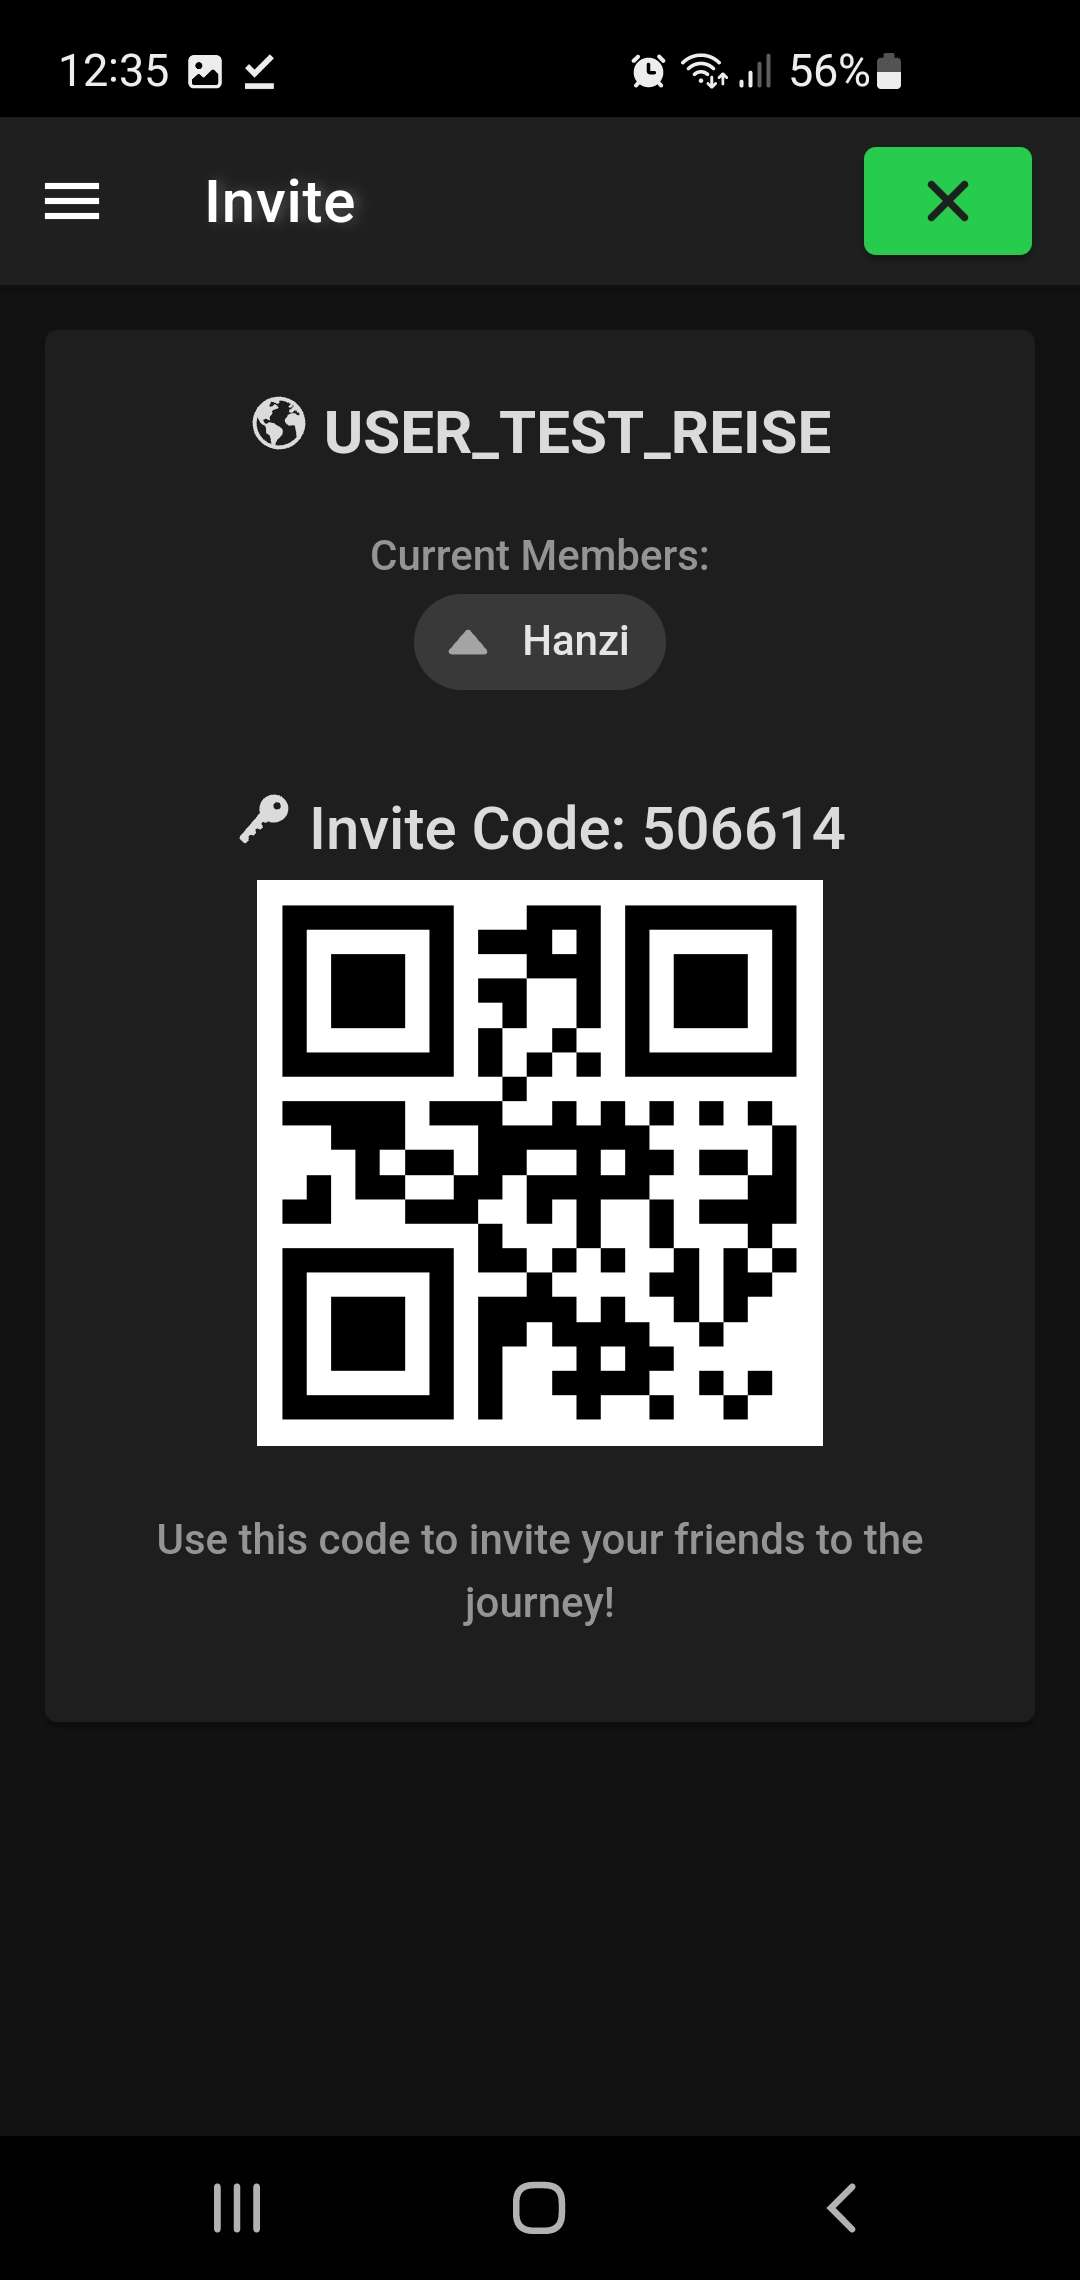
\includegraphics[width=0.3
		\textwidth]{img/user_test_invite}
		\caption[Usertest Einladung]{Usertesteinladung}
		%\captionsource{}
		\label{fig:user_test_invite}
	\end{figure}
	
	\begin{tabular}{|>{$\rhd$ }lrl|}
		\hline
		sehr gut  & \mybar{4}\\
		gut  & \mybar{0}\\
		ok               & \mybar{1}\\
		schlecht         & \mybar{1}\\
		\hline
	\end{tabular}
			
	\paragraph{Kommentar:}\ \\
	Ein Proband mit Bewertung \textbf{sehr gut} empfand die Anweisung als verwirrend. Ein Proband
mit Bewertung \textbf{ok} bemängelt eine fehlende deutsche Übersetzung. 

\newpage

	\subsubsection{Erstellen Sie in der Reise 'User\_Test\_Reise' eine Ausgabe, bei der Sie 50 € für ein Mittagessen mit Hanz und Marie gezahlt haben.}
	\begin{tabular}{|>{$\rhd$ }lrl|}
		\hline
		sehr gut  & \mybar{2}\\
		gut  & \mybar{2}\\
		ok               & \mybar{2}\\
		schlecht         & \mybar{0}\\
		\hline
	\end{tabular}
			
	\paragraph{Kommentar:}\ \\
	Ein Proband mit Bewertung \textbf{ok}:
	\begin{itemize}
		\item hätte Kategorie und Ausgabenbeteiligte fast übersprungen
		\item hat die Aufgabe zunächst missverstanden und sich nicht als Ausgabenbeteiligter eingetragen.
		\item wollte Teilnehmer mit in den Titel eingeben.
	\end{itemize}
	Ein Proband mit Bewertung \textbf{ok} hat den Titel vergessen.


	\subsubsection{Bearbeite Sie die Zahlung zu 85 €.}
	\begin{tabular}{|>{$\rhd$ }lrl|}
		\hline
		sehr gut  & \mybar{5}\\
		gut  & \mybar{0}\\
		ok               & \mybar{1}\\
		schlecht         & \mybar{0}\\
		\hline
	\end{tabular}
			
				
	\paragraph{Kommentar:}\ \\
	-

	\subsubsection{Lassen Sie sich die Schulden der Reise anzeigen.}
	\begin{tabular}{|>{$\rhd$ }lrl|}
		\hline
		sehr gut  & \mybar{4}\\
		gut  & \mybar{2}\\
		ok               & \mybar{0}\\
		schlecht         & \mybar{0}\\
		\hline
	\end{tabular}
	
	\paragraph{Kommentar:}\ \\
	Ein Proband mit Bewertung \textbf{gut} hatte zunächst in Ausgabe gesucht, dann aber die Seite
gefunden. Ein Proband mit Bewertung \textbf{gut} hat Zahlungen und Schulden verwechselt.

	\subsubsection{Vermerken Sie, dass Marie 5 € zurückgezahlt hat.}
	\begin{tabular}{|>{$\rhd$ }lrl|}
		\hline
		sehr gut  & \mybar{2}\\
		gut  & \mybar{2}\\
		ok               & \mybar{2}\\
		schlecht         & \mybar{0}\\
		\hline
	\end{tabular}
			
	\paragraph{Kommentar:}\ \\
	Zwei Probanden mit Bewertung \textbf{gut} und \textbf{ok} empfanden verwirrend, dass bei festhalten einer
Zahlung bereits der Betrag der Gesamtschulden eingetragen ist.

	\subsubsection{Erstellen Sie in der Reise 'User\_Test\_Reise' eine Ausgabe bei der Hanz für Sie beide ein Taxi am 03.01.23 für 100 € gezahlt hat.}
	\begin{tabular}{|>{$\rhd$ }lrl|}
		\hline
		sehr gut  & \mybar{5}\\
		gut  & \mybar{0}\\
		ok               & \mybar{1}\\
		schlecht         & \mybar{0}\\
		\hline
	\end{tabular}
			
	\paragraph{Kommentar:}\ \\
	Ein Proband mit Bewertung \textbf{ok} hat Beteiligte und Titel vergessen.

	\subsubsection{Lassen Sie sich die Schulden der Reise erneut anzeigen. Ändern Sie die Währung zu £.}
	\begin{tabular}{|>{$\rhd$ }lrl|}
		\hline
		sehr gut  & \mybar{6}\\
		gut  & \mybar{0}\\
		ok               & \mybar{0}\\
		schlecht         & \mybar{0}\\
		\hline
	\end{tabular}
			
	\paragraph{Kommentar:}\ \\
	-
	
	\subsubsection{Halten Sie fest, dass Sie Marie die Schulden zurückgezahlt haben.}
	\begin{tabular}{|>{$\rhd$ }lrl|}
		\hline
		sehr gut  & \mybar{5}\\
		gut  & \mybar{0}\\
		ok               & \mybar{0}\\
		schlecht         & \mybar{1}\\
		\hline
	\end{tabular}
			
	\paragraph{Kommentar:}\ \\
	Auf der Umfrageseite stand zeitweise Hanz anstelle von Marie, dieser besitzt aber zu diesem
Zeitpunkt keine Schulden.


	\subsubsection{Ändern Sie die Sortierung für die Ausgaben der Reise 'User\_Test\_Reise'.}
	\begin{tabular}{|>{$\rhd$ }lrl|}
		\hline
		sehr gut  & \mybar{5}\\
		gut  & \mybar{1}\\
		ok               & \mybar{0}\\
		schlecht         & \mybar{0}\\
		\hline
	\end{tabular}
			
	\paragraph{Kommentar:}\ \\
	Es wurde ein Bug festgestellt. Reise sowie Reiseliste aktualisieren sich nicht. Ausgaben werden
nicht eingefügt, sondern sind erst nach neu laden da. 
	
	\subsubsection{Löschen Sie alle Ausgaben der Reise 'User\_Test\_Reise'.}
	\begin{tabular}{|>{$\rhd$ }lrl|}
		\hline
		sehr gut  & \mybar{6}\\
		gut  & \mybar{0}\\
		ok               & \mybar{0}\\
		schlecht         & \mybar{0}\\
		\hline
	\end{tabular}
			
	\paragraph{Kommentar:}\ \\
	-
	
	\subsubsection{Archivieren Sie die von Ihnen erstellte Reise.}\label{Archivieren Sie die von Ihnen erstellte Reise.}
	\begin{tabular}{|>{$\rhd$ }lrl|}
		\hline
		sehr gut  & \mybar{0}\\
		gut  & \mybar{4}\\
		ok               & \mybar{0}\\
		schlecht         & \mybar{2}\\
		\hline
	\end{tabular}
			
	\paragraph{Kommentar:}\ \\
	Zwei Probanden mit Bewertung schlecht haben den Button nicht gefunden und hatten auch
keine Idee wo er sein könnte.
	
	\subsubsection{Loggen Sie sich aus der App aus.}
	\begin{tabular}{|>{$\rhd$ }lrl|}
		\hline
		sehr gut  & \mybar{5}\\
		gut  & \mybar{1}\\
		ok               & \mybar{0}\\
		schlecht         & \mybar{0}\\
		\hline
	\end{tabular}
			
	\paragraph{Kommentar:}\ \\
	-
	
\subsection{Fazit der Userteststudie}
Wir sind mit dem Ergebnis der Userteststudie zufrieden. Die Probanden sind für erstmaliges Nutzen der App gut zurechtgekommen. Aus dem Ergebnis von Anweisung \ref{Archivieren Sie die von Ihnen erstellte Reise.} leiten wir
Verbesserdungsbedarf ab, z. B. durch ein anderes Icon. Beim Archivieren-Button hatten wir
zeitweise ein passenderes Icon, aber Ionic bietet kein passendes Icon für die Umkehrfunktion zum entarchivieren daher hatten wir das Schloss-Icon verwendet.
Allgemein ein größeres Problem war die fehlende Validierung. Eine Validierung von Nutzereingaben war eigentlich einem Gruppenmitglied zugeteilt worden, dieses hat uns kurz vor Abgabe
verlassen. Eine Erkenntnis für unsere Gruppe daraus ist, dass man eine solche wichtige Aufgabe jemand geben sollte, der verantwortungsbewusst und verlässlich ist. Man sollte die Validierung
auf keinen Fall jemanden zuteilen, der trotz mehrfacher Hilfestellungen, vielen YouTube Tutorials, einer 90 min Vorlesung und einer 4-wöchigen Bearbeitungszeit nicht in der Lage ist ein
Inputtext auf einen vorhandenen Inhalt zu prüfen. 
Es war das erstmal, dass wir eine solche Studie durchgeführt haben und wir wurden in unserem vorherigen Studium für so etwas nicht ausgebildet. Für eine solche Studie selbst haben wir
gelernt, dass man die Anweisungen noch präziser formulieren sollte.

\section{Evaluation}
In diesem Kapitel wird evaluiert, inwiefern die Software die gestellten Anforderungen umsetzt. Dabei werden die funktionalen und nicht-funktionalen Anforderungen betrachtet.

\subsection{Funktionale Anforderungen}

\textbf{Use Case 1: Einen Account erstellen}\\
\begin{addmargin}{10pt}
\underline{Hauptszenario}: Alle Kriterien wurden erfüllt.\\
\underline{Ausnahmeszenarien}: Das Szenario 4b wurde nicht umgesetzt, da für die Passworteingabe keine Regelvalidierung umgesetzt wurde. Dementsprechend wird keine Fehlermeldung wie z.B. 'Das Passwort muss mindestens 8 Zeichen lang sein, einen Großbuchstaben und ein Sonderzeichen enthalten.' angezeigt. Dies wäre Aufgabe des Teammitglieds gewesen, das abgesprungen ist.\\
\end{addmargin}
\\
\textbf{Use Case 2: In Account einloggen}\\

\begin{addmargin}{10pt}
\underline{Hauptszenario}: Der Nutzer wird nicht wie Punkt 5 beschreibt auf seine aktive Reise weitergeleitet. Hier haben wir uns dazu entschieden, stattdessen auf die Liste aller aktiven Reisen weiterzuleiten, weil es als verwirrend empfunden wurde nach dem Login nicht in einer Form von Übersicht zu landen. Alle anderen Kriterien wurden erfüllt.\\
\underline{Alternativszenarien}: Alle Kriterien wurden erfüllt.\\
\underline{Ausnahmeszenarien}: Der Login-Button ist nicht wie gefordert ausgegraut, wenn der Nutzer eine ungültige E-Mail-Adresse eingibt. Dies wäre Aufgabe des Teammitglieds gewesen, das abgesprungen ist. Der Button ist lediglich ausgegraut, solange noch keine E-Mail-Adresse bzw. Passwort eingegeben wurde. Alle anderen Kriterien wurden erfüllt.\\
\end{addmargin}
\\
\textbf{Use Case 3: Eine Reise erstellen}\\

\begin{addmargin}{10pt}
\underline{Hauptszenario}: Alle Kriterien wurden erfüllt.\\
\underline{Ausnahmeszenarien}: Es können ungültige Reisezeiträume eingegeben werden (Enddatum liegt vor Startdatum). Dies wäre Aufgabe des Teammitglieds gewesen, das abgesprungen ist.\\
\end{addmargin}
\\
\textbf{Use Case 4: Eine Reise betreten}\\

\begin{addmargin}{10pt}
\underline{Hauptszenario}: Alle Kriterien wurden erfüllt.\\
\underline{Alternativszenarien}: Der QR-Scanner wurde nicht implementiert. Grund dafür war, dass wir das \href{https://ionicframework.com/docs/v3/native/qr-scanner/}{QR-Scanner Plugin} nicht lauffähig bekommen haben.\\
\underline{Ausnahmeszenarien}: Alle Kriterien wurden erfüllt.\\
\end{addmargin}
\\
\textbf{Use Case 5: Zahlung festhalten}\\

\begin{addmargin}{10pt}
\underline{Hauptszenario}: Alle Kriterien wurden erfüllt.\\
\underline{Alternativszenarien}: Der Nutzer kann ein Bild hochladen, allerdings nur Bilder aus dem Gerätespeicher und nicht per Kamera. Wir haben dafür die \href{https://ionicframework.com/docs/angular/your-first-app/taking-photos}{Camera API von Capacitor} verwendet. Die Kamera konnte geöffnet werden und ein Foto konnte ebenfalls geschossen werden, allerdings wurde das geschossene Foto nicht hochgeladen; diesen Fehler konnten wir nicht beheben.\\
\underline{Ausnahmeszenarien}: Der Nutzer kann negative Beträge eingeben, ohne dass die App dies verhindert oder meldet. Dies wäre Aufgabe des Teammitglieds gewesen, das abgesprungen ist.\\
\end{addmargin}
\\
\textbf{Use Case 6: Zahlung einsehen}\\

\begin{addmargin}{10pt}
\underline{Hauptszenario}: Alle Kriterien wurden erfüllt.\\
\end{addmargin}
\\
\textbf{Use Case 7: Schulden einsehen}\\

\begin{addmargin}{10pt}
\underline{Hauptszenario}: Alle Kriterien wurden erfüllt.\\
\underline{Alternativszenarien}: Alle Kriterien wurden erfüllt.\\
\end{addmargin}
\\
\textbf{Use Case 8: Reise archivieren}\\

\begin{addmargin}{10pt}
\underline{Hauptszenario}: Alle Kriterien wurden erfüllt.\\
\end{addmargin}
\\
\textbf{Use Case 9: Reisen einsehen}\\

\begin{addmargin}{10pt}
\underline{Hauptszenario}: Alle Kriterien wurden erfüllt.\\
\end{addmargin}
\\
Somit wurden bis auf die genannten Punkte alle funktionalen Anforderungen, die in Form von Use Cases formuliert wurden, umgesetzt.


\section{Nichtfunktionale Anforderungen}






\section{Anwenderdokumentation}



\subsection{Seitenerläuterung}

\subsubsection{Anmeldeseite}\label{Login}
\begin{figure}[H]
    \centering
    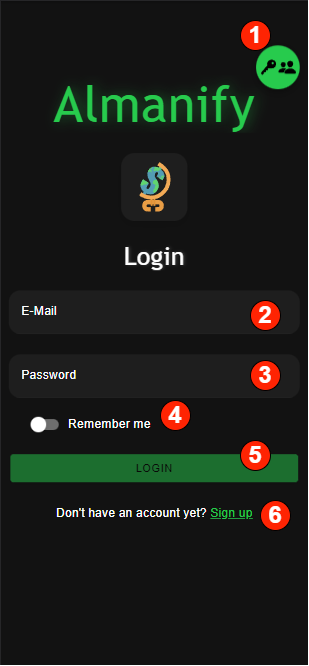
\includegraphics[width=0.3\textwidth]{img/pages_numbers/login.drawio}
    \caption[Login]{Login}
    %\captionsource{}
    \label{fig:Login}
\end{figure}
Auf dieser Seite kann sich der User anmelden.
\begin{enumerate}[label=\protect\circled{\arabic*}]
	\item Schnelllogin: ermöglicht das schnelle Anmelden mit verschiedenen Testuseren. (nur im Debugmodus vorhanden)
	\item Eingabelfeld für die E-Mailadresse des Nutzers mit der er sich registriert hat.
	\item Eingabelfeld für das Passwort des Nutzers.
	\item Remember me: der User kann auswählen ob er sich nach schließen der App erneut anmelden möchte.
	\item Button um sich einzuloggen.
	\item Wenn der Nutzer noch keinen Account hat gelangt er hier zur Registrierungsseite (Siehe \ref{Signup}).
\end{enumerate}

\subsubsection{Registrierungsseite}\label{Signup}
\begin{figure}[H]
    \centering
    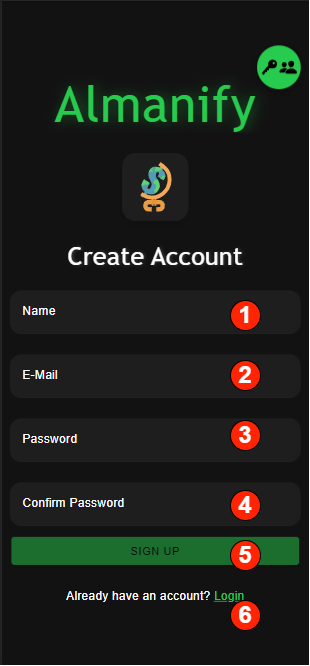
\includegraphics[width=0.3\textwidth]{img/pages_numbers/signup.drawio}
    \caption[Signup]{Signup}
    %\captionsource{}
    \label{fig:Signup}
\end{figure}
Auf dieser Seite kann sich der User registrieren.
\begin{enumerate}[label=\protect\circled{\arabic*}]
	\item Eingabelfeld für den Nutzername der den Mitreisenden später angezeigt wird.
	\item Eingabelfeld für die E-Mailadresse des Nutzers.
	\item Eingabelfeld für das Passwort des Nutzers.
	\item Eingabelfeld um das Passwort des Nutzers zu bestätigen.
	\item Button um sich zu registrieren.
	\item Wenn der Nutzer einen Account hat gelangt er hier zurück zu Loginseite (Siehe \ref{Login}).
\end{enumerate}

\subsubsection{Home}\label{Home}
\begin{figure}[H]
    \centering
    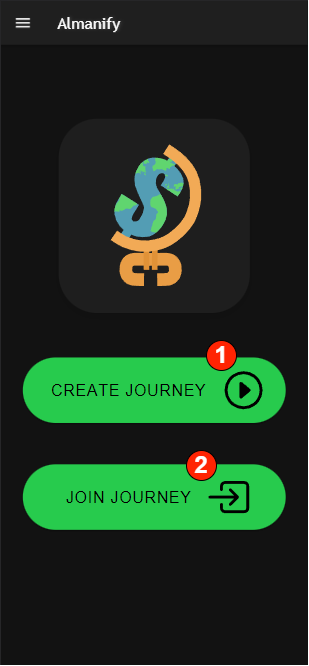
\includegraphics[width=0.3\textwidth]{img/pages_numbers/home.drawio}
    \caption[Home]{Home}
    %\captionsource{}
    \label{fig:Home}
\end{figure}
Auf diese Seite gelangt der User nach Login, wenn keine aktive Reise vorhanden ist.
\begin{enumerate}[label=\protect\circled{\arabic*}]
	\item Button zum Erstellen einer neuen Reise: der Nutzer gelangt zur Reiseerstellenseite (Siehe \ref{Journey-Editor}).
	\item Button zum Beitreten einer existierenden Reise: der Nutzer gelangt zur Reisebeitretenseite (Siehe \ref{TODO}).
\end{enumerate}

\subsubsection{Reisebearbeiten/erstellen}\label{Journey-Editor}
\begin{figure}[H]
    \centering
    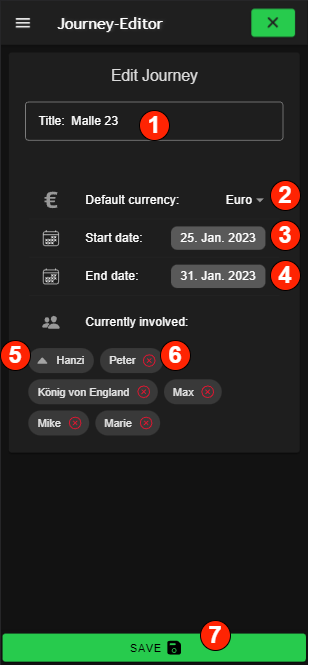
\includegraphics[width=0.3\textwidth]{img/pages_numbers/journey-editor.drawio}
    \caption[Journey-Editor]{Journey-Editor}
    %\captionsource{}
    \label{fig:Journey-Editor}
\end{figure}
Auf dieser Seite kann der User eine Reise erstellen oder bearbeiten. Entsprechend der Situation ist der Titel  "`New Journey"' oder "`Edit Journey"'.
\begin{enumerate}[label=\protect\circled{\arabic*}]
	\item Eingabefeld um der Reise einen Titel zugeben der später für alle Angezeigt wird.
	\item Dropdown zur Auswahl einer Standardwährung auf der Reise.
	Die Standardwährung ist später beim Erstellen von Zahlungen voreingestellt.
	\item Öffnet Modal zur Wahl des Startdatums der Reise.
	\item Öffnet Modal zur Wahl des Enddatums der Reise.
	\item Ersteller einer Reise wird mit Dreieckicon markiert.
	\item Nicht-Ersteller einer Reise können mit x-Button aus der Reise gekickt werde.
	\item Button zum Speichern des Eintrags.
\end{enumerate}

\subsubsection{Detailansicht einer Reise}\label{Journey-Details}
\begin{figure}[H]
    \centering
    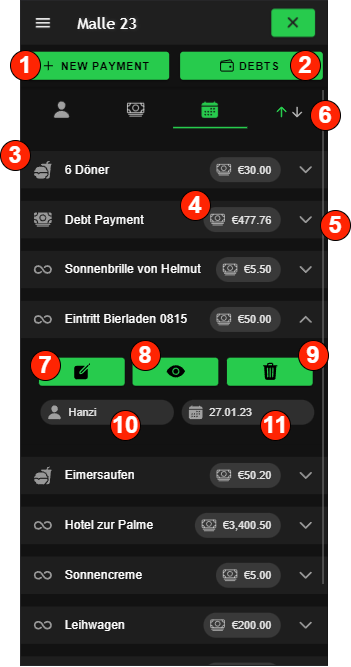
\includegraphics[width=0.3\textwidth]{img/pages_numbers/journey-details.drawio}
    \caption[Journey-Details]{Journey-Details}
    %\captionsource{}
    \label{fig:Journey-Details}
\end{figure}
Auf dieser Seite hat der Nutzer eine Übersicht aller Zahlungen einer Reise.
Der Nutzer gelangt nach Login auf diese Seite, wenn es sich um die aktuellste Reise handelt.
\begin{enumerate}[label=\protect\circled{\arabic*}]
	\item Button zum Erstellen einer neue Zahlung: der Nutzer gelangt zur Zahlungerstellenseite (Siehe \ref{payment-details_(edit-mode)}).
	\item Button zur Schuldenübersicht: der Nutzer gelangt zu Schuldenübersicht der Reise (Siehe \ref{debt-calculator_(owe)} und \ref{debt-calculator_(owed)}).
	\item Icon sagt über Kategorie der Zahlung aus (siehe Tabelle \ref{Tab:paymentcategories}).
	\item Betrag und Währung einer Zahlung.
	\item Öffnen von weiteren Optionen zu einer Zahlung.
	\item Zahlung können auf- und absteigend anhand des Zahlers, des Betrags und des Zahldatums sortiert werden.
	\item Button zum Bearbeiten einer Zahlung: der Nutzer gelangt zur Zahlungbearbeitenseite  (Siehe \ref{payment-details_(edit-mode)}).
	\item Button zu Details einer Ausgab: der Nutzer gelangt zur Detailansicht einer Zahlung  (Siehe \ref{payment-details}).
	\item Button zum Löschen einer Zahlung.
	\item Nutzername des Zahlers.
	\item Zahldatum.
\end{enumerate}

\begin{table}[H]
\caption{Zahlungskategorien}
\begin{tabularx}{0.95\textwidth}{ |X|X|X| }
\hline
\rowcolor{gray} \textbf{Bezeichnung} & \textbf{Icon} & Beschreibung\\
\hline
accommodation & 
\includegraphics[width=0.05\textwidth]{paymentcategories/bed.pdf} &
Ausgaben für Unterkunft. \\
\hline
	Food\&Trink & 
\includegraphics[width=0.05\textwidth]{paymentcategories/fast-food.pdf} & Ausgaben für Essen und Trinken. \\
\hline
	entertaiment & 
\includegraphics[width=0.05\textwidth]{paymentcategories/game-controller.pdf} & Ausgaben für Unterhaltung.\\
\hline
	transfer & 
\includegraphics[width=0.05\textwidth]{paymentcategories/airplane.pdf}& Ausgaben die Transportmittel betreffen. \\
\hline
	repayment & 
\includegraphics[width=0.05\textwidth]{paymentcategories/cash.pdf} & Rückzahlung von Schulden an andere Mitreisende. \\
\hline
	other & 
\includegraphics[width=0.05\textwidth]{paymentcategories/infinite.pdf} & alles was in keine andere Kategorie passt.\\
\hline
\end{tabularx}
\label{Tab:paymentcategories}
\end{table}

\subsubsection{Liste der beigetretenen Reisen}\label{Journey-List}
\begin{figure}[H]
    \centering
    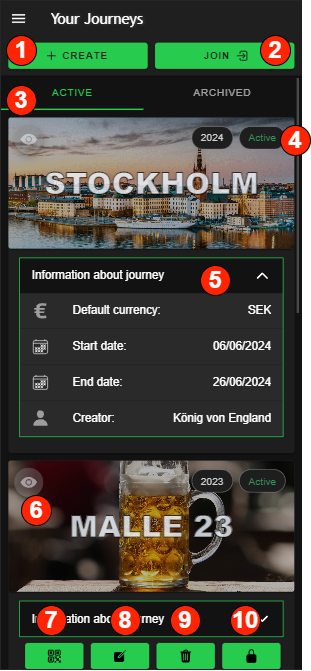
\includegraphics[width=0.3\textwidth]{img/pages_numbers/journey-list.drawio}
    \caption[Journey-List]{Journey-List}
    %\captionsource{}
    \label{fig:Journey-List}
\end{figure}
Auf dieser Seite hat der Nutzer eine Übersicht aller beigetretenen Reisen.
\begin{enumerate}[label=\protect\circled{\arabic*}]
	\item Button zum Erstellen einer neuen Reise: der Nutzer gelangt zur Reiseerstellenseite  (Siehe \ref{Journey-Editor}).
	\item Auswahl zwischen aktiven und archivierten Reisen.
	\item Anzeige ob es sich um eine aktive oder archivierte Reise handelt.
	\item Button zu Details einer Reise: der Nutzer gelangt zu einer Listenansicht aller Reisezahlungen  (Siehe \ref{Journey-Details}).
	\item Der Nutzer bekommt das Einladungsmodal angezeigt (Siehe \ref{invite-modal}).
	\item Button zum Reisebearbeiten: der Nutzer gelangt zur Reisebearbeitenseite (Siehe \ref{Journey-Editor}).
	\item Button zum Löschen einer Reise.
	\item Button zum Archivieren einer Reise.
	\item Titel der Reise als Vektorbild, kann vom Nutzer durch eigenes Bild ersetzt werden.
	\item Ist der Nutzer nicht Ersteller einer Reise wird ihm nur der Button zu den Details einer Reise angezeigt.
\end{enumerate}

\subsubsection{Details einer Zahlung}\label{payment-details}
\begin{figure}[H]
    \centering
    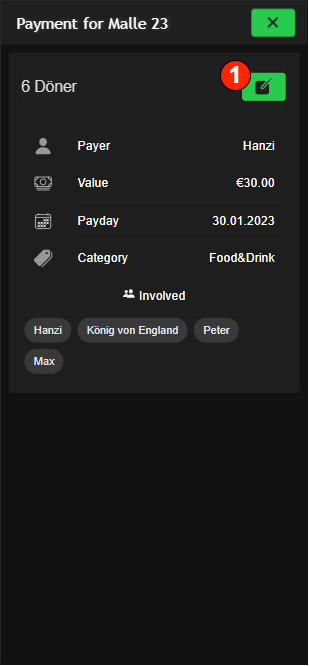
\includegraphics[width=0.3\textwidth]{img/pages_numbers/payment-details.drawio}
    \caption[Payment-Details]{Payment-Details}
    %\captionsource{}
    \label{fig:payment-details}
\end{figure}
Auf dieser Seite sieht der Nutzer alle Infos zu einer Zahlung.
\begin{enumerate}[label=\protect\circled{\arabic*}]
	\item Wechseln in den Bearbeitenmodus (Siehe \ref{payment-details_(edit-mode)}).
\end{enumerate}

\subsubsection{Details einer Zahlung beim erstellen/bearbeiten}\label{payment-details_(edit-mode)}
\begin{figure}[H]
    \centering
    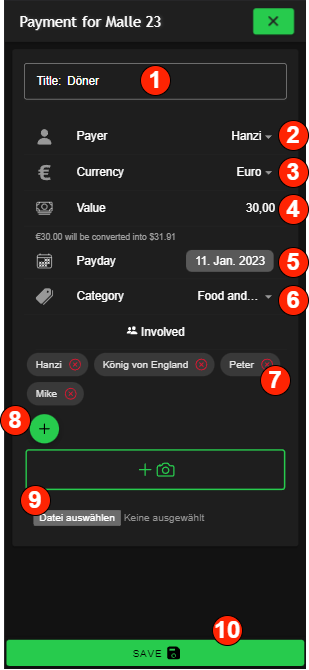
\includegraphics[width=0.3\textwidth]{img/pages_numbers/payment-details_(edit-mode).drawio}
    \caption[Payment-Details (Edit-Mode)]{Payment-Details (Edit-Mode)}
    %\captionsource{}
    \label{fig:payment-details_(edit-mode)}
\end{figure}
Auf dieser Seite kann der Nutzer die Informationen zu einer Zahlung erstellen oder bearbeiten.
\begin{enumerate}[label=\protect\circled{\arabic*}]
	\item Titel der Zahlung
	\item Dropdown mit allen Reisebeteiligten zur Auswahl des Zahlers. Der Ersteller einer Zahlung ist hier 			vorausgewählt.
	\item Dropdown für die Wahl der Währung. Die Standartwährung der Reise ist beim Erstellen vorausgewählt.
	\item Input für den Betrag der Zahlung.
	\item Öffnet Modal um den Zahltag auszuwählen.
	\item Dropdown zur Auswahl der Zahlungskategorie.
	\item Durch den x-Button können Nutzer als Zahlungsverursacher entfernt werden.
	\item Mit dem Plus-Button können einzelne Nutzer oder alle Nutzer hinzugefügt werden. Zusätzlich gibt es die Möglichkeit alle Nutzer zu entfernen.
	\item Button um die Kamera zu öffnen und um ein Bild der Rechnung festzuhalten.
	\item Button zum Speichern des Eintrags.
\end{enumerate}


\subsubsection{Schuldenansicht bei Guthaben}\label{debt-calculator_(owed)}
\begin{figure}[H]
    \centering
    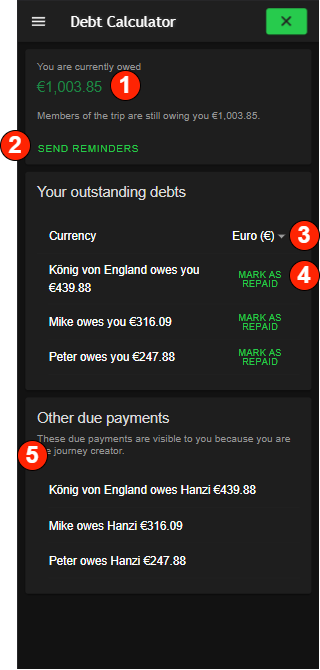
\includegraphics[width=0.3\textwidth]{img/pages_numbers/debt-calculator_(owed).drawio}
    \caption[Debt-Calculator (Owed)]{Debt-Calculator (Owed)}
    %\captionsource{}
    \label{fig:debt-calculator_(owed)}
\end{figure}
Auf dieser Seite sieht der Nutzer sein Guthaben bzw. seine Schulden gegenüber anderen (Siehe \ref{debt-calculator_(owe)}).
\begin{enumerate}[label=\protect\circled{\arabic*}]
	\item Der Betrag, was einem die Mitreisenden noch schulden.
	\item Sendet eine Push-Nachricht als Erinnerung an alle Schuldner.
	\item Öffnet Zahlungerstellen um den gezahlten Betrag festzuhalten.
	\item Als Reiseersteller hat man zusätzlich die Übersicht über alle offene Schulden einer Reise
\end{enumerate}

\subsubsection{Schuldenansicht bei Schulden}\label{debt-calculator_(owe)}
\begin{figure}[H]
    \centering
    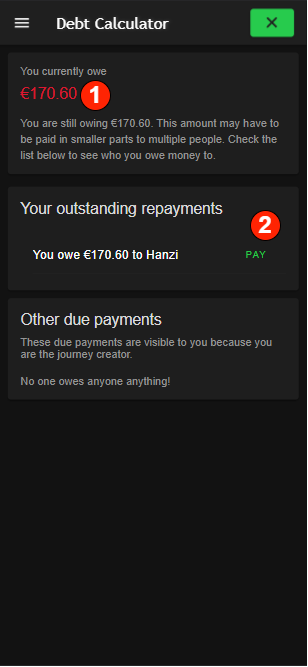
\includegraphics[width=0.3\textwidth]{img/pages_numbers/debt-calculator_(owe).drawio}
    \caption[Debt-Calculator (Owe)]{Debt-Calculator (Owe)}
    %\captionsource{}
    \label{fig:debt-calculator_(owe)}
\end{figure}
\begin{enumerate}[label=\protect\circled{\arabic*}]
	\item Der Betrag, was man den Mitreisenden noch schuldet.
	\item Öffnet Zahlungerstellen mit vor gefüllten Werten um die Übermittlung einer Zahlung festzuhalten.
\end{enumerate}

\subsubsection{Einladungsmodal}\label{invite-modal}
\begin{figure}[H]
    \centering
    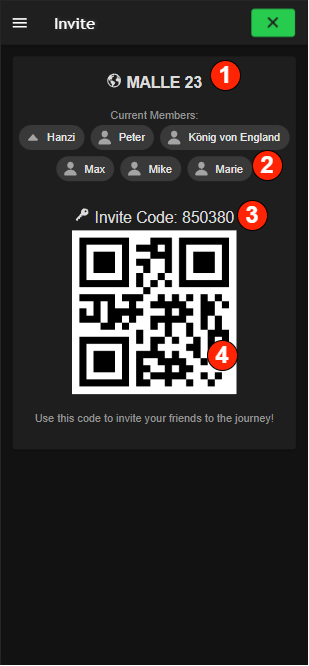
\includegraphics[width=0.3\textwidth]{img/pages_numbers/invite-modal.drawio}
    \caption[Invite-Modal]{Invite-Modal}
    %\captionsource{}
    \label{fig:invite-modal}
\end{figure}
Auf dieser Seite erhält der Reiseersteller alle Informationen um weitere Nutzer in seine Reise einzuladen.
\begin{enumerate}[label=\protect\circled{\arabic*}]
	\item Title der Reise für die eingeladen wird.
	\item Liveansicht aller der Reise beigetretenen Nutzer.
	\item Invitecode zur Eingabe auf der Reisebeitrittseite um der Reise beizutreten.
	\item Der Invitecode als QR-Code zum einfachen Scannen auf der Reisebeitrittseite um der Reise beizutreten.
\end{enumerate}

\subsubsection{Optionen}\label{options}
\begin{figure}[H]
    \centering
    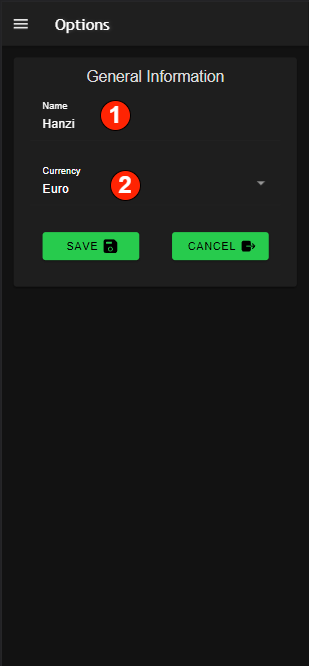
\includegraphics[width=0.3
    \textwidth]{img/pages_numbers/options.drawio}
    \caption[Options]{Options}
    %\captionsource{}
    \label{fig:options}
\end{figure}
Auf dieser Seite kann der Nutzer seine Daten anpassen.
\begin{enumerate}[label=\protect\circled{\arabic*}]
	\item Ändern des Nutzernamens.
	\item Anpassen der Wunschwährung in der Schulden angezeigt werden sollen.
\end{enumerate}


\subsection{Sitemap}

\begin{figure}[H]
    \centering
    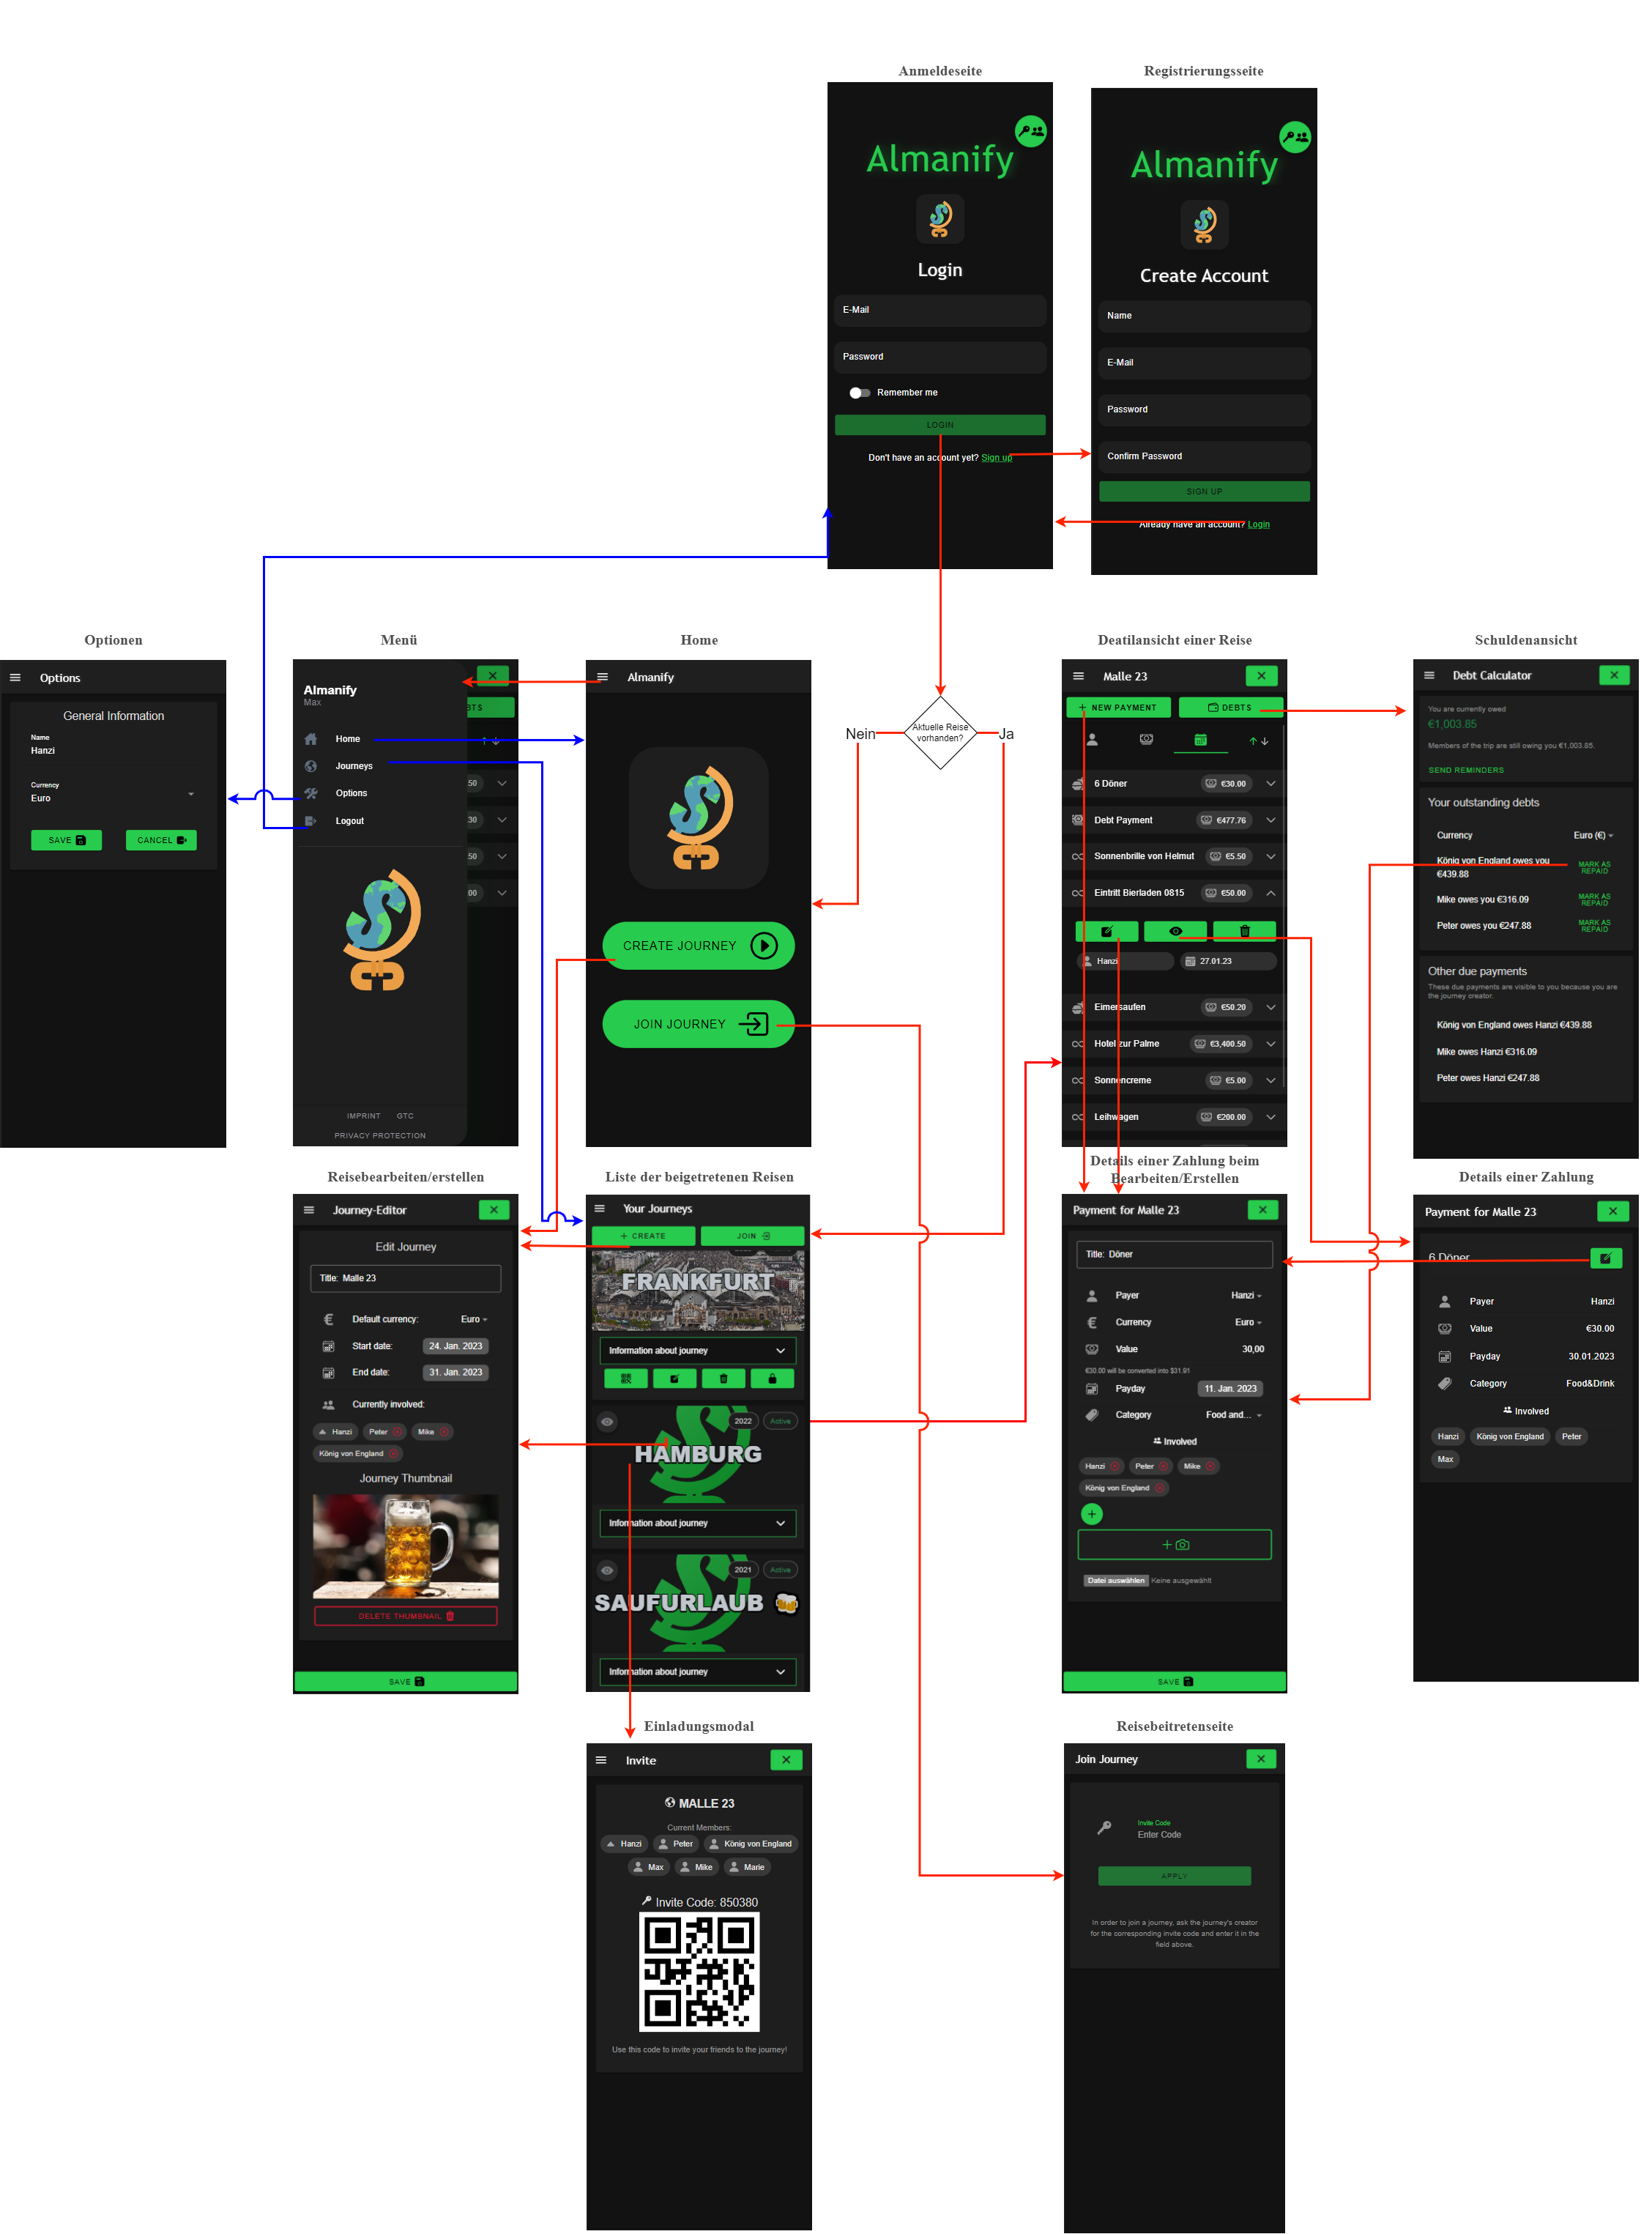
\includegraphics[width=\textwidth]{img/Sitemap}
    \caption[Sitemap]{Sitemap}
    %\captionsource{}
    \label{fig:Sitemap}
\end{figure}
\clearpage

%Römische Seitennummerierung
\pagenumbering{Roman}
\setcounter{page}{1}

% ================================
% Falls nicht verwendet bitte entsprechend auskommentieren
% ================================
%Anhang
%\include{chapter/anhang}
\pagebreak

%Abbildungsverzeichnis
%\listoffigures
\pagebreak

%Tabellenverzeichnis
%\listoftables
\pagebreak

%Literaturverzeichnis
\bibliographystyle{literature/bibtex/IEEEtran}
\bibliography{literature/literature}

\end{document}
